\documentclass{article}
\usepackage[paperwidth=7.16in,paperheight=2.40in,margin=0in]{geometry}
\usepackage{times}
\usepackage{tikz}
\usetikzlibrary{arrows.meta,positioning,calc,fit,backgrounds}
\pagestyle{empty}

\definecolor{rcEBH}{RGB}{0,114,178}
\definecolor{rcBase}{RGB}{213,94,0}
\definecolor{rcNeutral}{RGB}{107,114,128}
\definecolor{rcDark}{RGB}{17,24,39}
\definecolor{rcScreen}{RGB}{255,247,237}
\definecolor{rcInfer}{RGB}{239,246,255}
\definecolor{rcHold}{RGB}{248,250,252}

\begin{document}
\noindent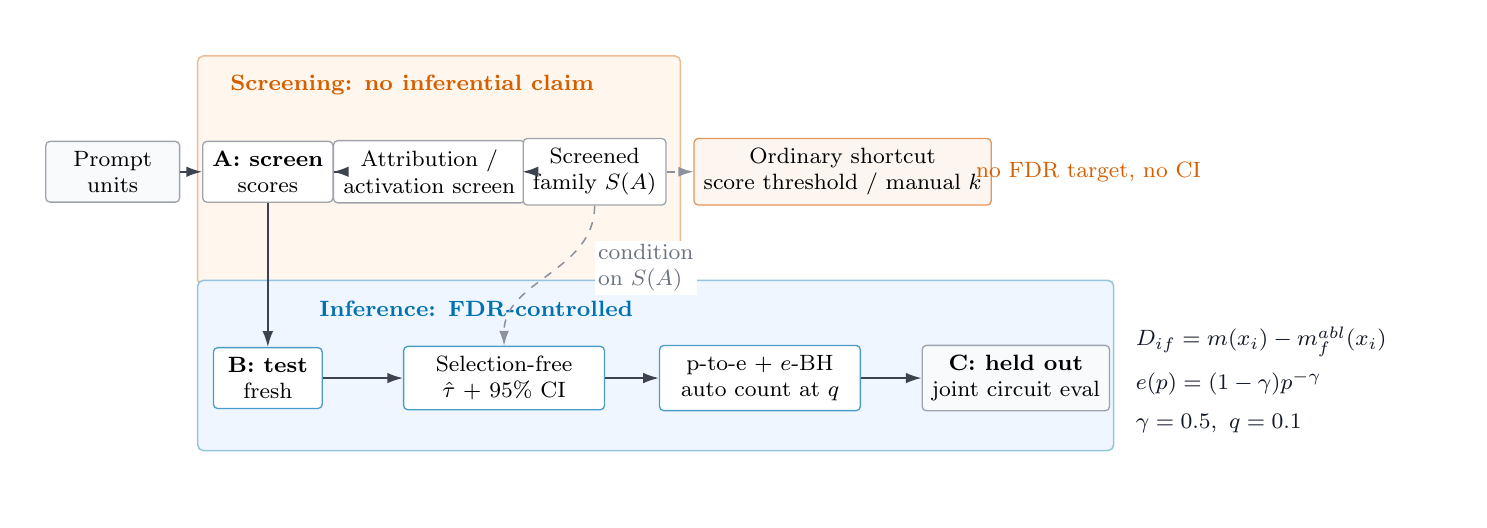
\begin{tikzpicture}[
  x=1cm,y=1cm,
  >=Latex,
  box/.style={draw=rcNeutral!65, line width=0.48pt, rounded corners=1.5pt,
    fill=white, align=center, inner sep=3.5pt, font=\footnotesize},
  stage/.style={box, minimum height=0.72cm},
  method/.style={box, draw=rcEBH!70, fill=white, minimum height=0.72cm},
  side/.style={box, draw=rcBase!65, fill=rcBase!6, minimum height=0.68cm},
  region/.style={rounded corners=2pt, line width=0.55pt, inner sep=4pt},
  arrow/.style={-{Latex[length=2.0mm,width=1.35mm]}, line width=0.62pt, draw=rcDark!82},
  weak/.style={-{Latex[length=1.9mm,width=1.25mm]}, line width=0.55pt, draw=rcNeutral!78, dashed}
]
\path[use as bounding box] (0,0.55) rectangle (18.18,6.55);

% Colored process regions.
\node[region, draw=rcBase!42, fill=rcScreen, fit={(2.30,3.42) (8.15,6.05)}] (screenzone) {};
\node[anchor=west, font=\footnotesize\bfseries, text=rcBase] at (2.45,5.82)
  {Screening: no inferential claim};
\node[region, draw=rcEBH!42, fill=rcInfer, fit={(2.30,1.32) (13.65,3.20)}] (inferzone) {};
\node[anchor=west, font=\footnotesize\bfseries, text=rcEBH] at (3.58,2.98)
  {Inference: FDR-controlled};

% Main split and screening line.
\node[stage, minimum width=1.70cm, fill=rcHold] (prompt) at (1.08,4.72)
  {Prompt\\units};
\node[stage, minimum width=1.38cm] (a) at (3.05,4.72)
  {\textbf{A: screen}\\scores};
\node[stage, minimum width=2.10cm] (attrib) at (5.10,4.72)
  {Attribution /\\activation screen};
\node[stage, minimum width=1.70cm] (family) at (7.20,4.72)
  {Screened\\family $S(A)$};

\draw[arrow] (prompt) -- (a);
\draw[arrow] (a) -- (attrib);
\draw[arrow] (attrib) -- (family);

% Shortcut branch.
\node[side, minimum width=2.85cm] (shortcut) at (10.35,4.72)
  {Ordinary shortcut\\score threshold / manual $k$};
\draw[weak] (family.east) -- (shortcut.west);
\node[anchor=west, font=\footnotesize, text=rcBase] at (11.92,4.72)
  {no FDR target, no CI};

% Inference line.
\node[method, minimum width=1.38cm] (b) at (3.05,2.10)
  {\textbf{B: test}\\fresh};
\node[method, minimum width=2.55cm] (infer) at (6.05,2.10)
  {Selection-free\\$\hat{\tau}$ + 95\% CI};
\node[method, minimum width=2.55cm] (ebh) at (9.30,2.10)
  {p-to-e + $e$-BH\\auto count at $q$};
\node[stage, minimum width=2.10cm, fill=rcHold] (c) at (12.55,2.10)
  {\textbf{C: held out}\\joint circuit eval};

\draw[arrow] (a.south) to[out=-90,in=90] (b.north);
\draw[arrow] (b) -- (infer);
\draw[arrow] (infer) -- (ebh);
\draw[arrow] (ebh) -- (c);

% Conditioning loop.
\draw[weak] (family.south) to[out=-90,in=90] (infer.north);
\node[font=\footnotesize,align=left,fill=white,inner sep=1.2pt,text=rcNeutral]
  at (7.85,3.50) {condition\\on $S(A)$};

% Compact estimand/e-value hint, kept outside the main boxes.
\node[anchor=west, font=\footnotesize, text=rcDark] at (13.95,2.56)
  {$D_{if}=m(x_i)-m_f^{abl}(x_i)$};
\node[anchor=west, font=\footnotesize, text=rcDark] at (13.95,2.04)
  {$e(p)=(1-\gamma)p^{-\gamma}$};
\node[anchor=west, font=\footnotesize, text=rcDark] at (13.95,1.52)
  {$\gamma=0.5,\ q=0.1$};

\end{tikzpicture}
\end{document}
